% Options for packages loaded elsewhere
\PassOptionsToPackage{unicode}{hyperref}
\PassOptionsToPackage{hyphens}{url}
\PassOptionsToPackage{dvipsnames,svgnames,x11names}{xcolor}
\documentclass[
  12pt,
]{article}
\usepackage{xcolor}
\usepackage[margin=1in]{geometry}
\usepackage{amsmath,amssymb}
\setcounter{secnumdepth}{5}
\usepackage{iftex}
\ifPDFTeX
  \usepackage[T1]{fontenc}
  \usepackage[utf8]{inputenc}
  \usepackage{textcomp} % provide euro and other symbols
\else % if luatex or xetex
  \usepackage{unicode-math} % this also loads fontspec
  \defaultfontfeatures{Scale=MatchLowercase}
  \defaultfontfeatures[\rmfamily]{Ligatures=TeX,Scale=1}
\fi
\usepackage{lmodern}
\ifPDFTeX\else
  % xetex/luatex font selection
\fi
% Use upquote if available, for straight quotes in verbatim environments
\IfFileExists{upquote.sty}{\usepackage{upquote}}{}
\IfFileExists{microtype.sty}{% use microtype if available
  \usepackage[]{microtype}
  \UseMicrotypeSet[protrusion]{basicmath} % disable protrusion for tt fonts
}{}
\makeatletter
\@ifundefined{KOMAClassName}{% if non-KOMA class
  \IfFileExists{parskip.sty}{%
    \usepackage{parskip}
  }{% else
    \setlength{\parindent}{0pt}
    \setlength{\parskip}{6pt plus 2pt minus 1pt}}
}{% if KOMA class
  \KOMAoptions{parskip=half}}
\makeatother
\usepackage{graphicx}
\makeatletter
\newsavebox\pandoc@box
\newcommand*\pandocbounded[1]{% scales image to fit in text height/width
  \sbox\pandoc@box{#1}%
  \Gscale@div\@tempa{\textheight}{\dimexpr\ht\pandoc@box+\dp\pandoc@box\relax}%
  \Gscale@div\@tempb{\linewidth}{\wd\pandoc@box}%
  \ifdim\@tempb\p@<\@tempa\p@\let\@tempa\@tempb\fi% select the smaller of both
  \ifdim\@tempa\p@<\p@\scalebox{\@tempa}{\usebox\pandoc@box}%
  \else\usebox{\pandoc@box}%
  \fi%
}
% Set default figure placement to htbp
\def\fps@figure{htbp}
\makeatother
% definitions for citeproc citations
\NewDocumentCommand\citeproctext{}{}
\NewDocumentCommand\citeproc{mm}{%
  \begingroup\def\citeproctext{#2}\cite{#1}\endgroup}
\makeatletter
 % allow citations to break across lines
 \let\@cite@ofmt\@firstofone
 % avoid brackets around text for \cite:
 \def\@biblabel#1{}
 \def\@cite#1#2{{#1\if@tempswa , #2\fi}}
\makeatother
\newlength{\cslhangindent}
\setlength{\cslhangindent}{1.5em}
\newlength{\csllabelwidth}
\setlength{\csllabelwidth}{3em}
\newenvironment{CSLReferences}[2] % #1 hanging-indent, #2 entry-spacing
 {\begin{list}{}{%
  \setlength{\itemindent}{0pt}
  \setlength{\leftmargin}{0pt}
  \setlength{\parsep}{0pt}
  % turn on hanging indent if param 1 is 1
  \ifodd #1
   \setlength{\leftmargin}{\cslhangindent}
   \setlength{\itemindent}{-1\cslhangindent}
  \fi
  % set entry spacing
  \setlength{\itemsep}{#2\baselineskip}}}
 {\end{list}}
\usepackage{calc}
\newcommand{\CSLBlock}[1]{\hfill\break\parbox[t]{\linewidth}{\strut\ignorespaces#1\strut}}
\newcommand{\CSLLeftMargin}[1]{\parbox[t]{\csllabelwidth}{\strut#1\strut}}
\newcommand{\CSLRightInline}[1]{\parbox[t]{\linewidth - \csllabelwidth}{\strut#1\strut}}
\newcommand{\CSLIndent}[1]{\hspace{\cslhangindent}#1}
\setlength{\emergencystretch}{3em} % prevent overfull lines
\providecommand{\tightlist}{%
  \setlength{\itemsep}{0pt}\setlength{\parskip}{0pt}}
\usepackage{setspace} \setstretch{1.15} \usepackage{float} \floatplacement{figure}{t}
\usepackage{bookmark}
\IfFileExists{xurl.sty}{\usepackage{xurl}}{} % add URL line breaks if available
\urlstyle{same}
\hypersetup{
  colorlinks=true,
  linkcolor={cyan},
  filecolor={Maroon},
  citecolor={Blue},
  urlcolor={cyan},
  pdfcreator={LaTeX via pandoc}}

\title{\large Assessing Ranking Fidelity of Competition Structures via
Weighted Mutual Information}
\author{}
\date{\vspace{-2.5em}}

\begin{document}
\maketitle
\begin{abstract}
We evaluate multiple competitions structures to assess their
effectiveness in accurately reproducing the true underlying ranking of
participating teams. Using repeated simulations for each structure, we
compare teams' true performance ranks to their simulated outcomes. To
quantify the accuracy of each format, we calculate weighted mutual
information between true and simulated rankings across a large number of
replicates. ``Salient'' weights are applied to look at only the top i
out of n total teams/competitors in a given competition structure. This
information-theoretic approach allows us to objectively compare formats
and identify which structures most effectively preserve rank order.
Results are visualized through comparative plots, providing clear
insights into the trade-offs and strengths of each competition design.\\

\vspace{2mm} \textbar{} Keywords: tournament structures, mutual
information
\end{abstract}

\section{Introduction}\label{introduction}

There are hundreds of different competitions structures that dictate how
a set of teams compete against each other to determine an overall
ranking. Common structures include bracket tournaments where if a team
wins their competition they advance to the next round. Bracket
tournaments can be run as single elimination where competitors advance
or are eliminated based on a single match (e.g.~NCAA College Basketball
Tournament, National Football League (NFL) playoffs, major tennis
tournaments) or where each round is contested as a best of \(k\) series
(e.g.~\(k\) = 7: National Basketball Association (NBA) playoffs,
National Hockey League (NHL) playoffs, \(k\) varies by round: Major
League Baseball (MLB), Women's National Basketball Association (WNBA))
and the series winner advance while the series loser is eliminated.
Additional styles of the bracket tournaments include variations where
competitors are not eliminated after a single loss such as double
elimination tournaments where competitors continue until they have lost
twice. Within double elimination tournament, there are several
variations. For instance, the NCAA College Wrestling tournament is a
double elimination tournament, however, if a competitor loses a match
they fall into the consolation bracket and the best they can finish
after a loss before the finals is 3rd place making this not a ``true''
double elimination format. Olympic judo uses a variant of this system
with single elimination until the quarterfinals followed by a
consolation bracket consisting of the four quarterfinal losers who still
have a chance for a bronze medal\footnote{in Olympic judo they award two
  bronze medals to the two competitors who each win their side of the
  consolation bracket}.

``True'' double elimination - a bracket tournament where a competitor
can still finish ranked first as long as a competitor has not lost two
games - is used in NCAA baseball and softball for certain rounds in
their postseason. Additional variants of double elimination include
double elimination brackets with a ``true third'' match which includes
an additional match contested between the competitors ranked 2nd (loser
of the finals) and 3rd (winner of the consolation bracket) at the end of
the tournament \emph{if they have not already competed against each
other}. There is also a variation of double elimination where only those
competitors who have lost to a competitor that makes the finals are
placed into the consolation bracket and given the chance to compete for
third place. This style of competition is used in Olympic wrestling
(both freestyle and Greco-Roman)\footnote{As in Olympic judo, Olympic
  wrestling also award two bronze medals to the winners of each side of
  the consolation bracket}.

In bracket style competitions, only a handful of the match-ups that are
possible actually occur. When every possible competitive pairing occurs,
this is referred to as a round-robin structure where every competitor
plays every other competitor the same number of times. Single
round-robin, where was possible match-up occurs exactly once, is used
in, for examples, the group stage of the FIFA World Cup to create a
ranking to determine which teams advance to the next round. Double
round-robin, where each possible pairing occurs twice, is used in
association football in English Premier League (EPL) and in chess during
the FIDE candidates tournament (a tournament that decides who will
challenge the world champion). For the sake of brevity, we review only a
small number of possible competition structures, but the interested
reader can find a more complete list of competition structures in
Devriesere and Goossens (\citeproc{ref-Goosens2024}{2025}), Appleton
(\citeproc{ref-Appleton1995-zn}{1995}) and Csato
(\citeproc{ref-Csato2021}{2021}).

A natural question of interest after reviewing different types of
competition structures is: which competition structure is best? As with
most complicated questions, the answer is ``it depends''. One
commonsense conceptualization for the best competition structure is that
the final rankings produced by a competition structure should closely
match the true rankings of the strength of the competitors. That is, a
good competition structure should rank the true best team first, the
true second best team second, and so on, until finally ranking the true
worst team last. We refer to this property of a competition structure as
the efficacy of the structure (Lasek and Gagolewski
(\citeproc{ref-Lasek2018-de}{2018}), Sziklai, Biró, and Csató
(\citeproc{ref-Sziklai2022-kf}{2022})). If one were only interested in
correctly ranking the true best competitor as first, with the ranks of
the remaining competitors viewed as inconsequential, we refer to this
here are effectivity (Glenn (\citeproc{ref-Glenn1960-mn}{1960})). While
there are many competition structures where efficacy and effectivity are
useful measures\footnote{efficacy is a useful measure for the EPL, for
  example, as the ranking of the teams matters at both the high end
  (i.e.~entry into special tournaments) and the low end (i.e.~relegation
  status) and effectivity is a useful measure for the NCAA College
  Basketball tournament (i.e.~main goal is to crown a champion)}, there
are many other competitions where the correct ranking of more than one
competitor, but not all the competitors is of import. For instance, in
Olympic competition, the goal of a competition structure is to correctly
rank the top 3 competitors to award gold, silver, and bronze medals
to\footnote{Some sports award two bronze medals (e.g.~wrestling, judo,
  boxing, tae kwon do)}. In many American sports, for instance the NFL,
the goal of the competition structure of the regular season is to rank
the top 7 teams in each conference to choose the playoff teams with the
ranking of the teams 8 through 16 in each conference inconsequential in
determining a Super Bowl champion\footnote{The ranking of teams outside
  of the playoffs does matter for draft purposes though}. We coin the
term ``salient ranks'' to refer to the ranks of a competition structure
that matter. That is the ranks 1, 2, and 3 in Olympic competition are
the salient ranks in that competition structure. In this notation,
efficacy is a measure with with salient ranks 1 through \(n\) where
\(n\) is the number of competitors, and effectivity is a measure where 1
is the only salient rank.\\

If the only goal of a competition structure was high efficacy of the
salient ranks, the best way to achieve this would be to play each pair
of possible match ups of competitors as many times as possible. Of
course, this is impossible due to many factors including time
constraints, cost constraints, and wear and tear on competitors in high
impact sports (e.g.~boxing, American football, etc.). In addition,
competitions where the true best team is guaranteed or nearly guaranteed
to win may be less appealing to fans and may drive down demand as
discussed in Johnson and Fort (\citeproc{ref-Johnson2022-wz}{2022}).

In light of this, many different competition structures have been
proposed, several of which are mentioned previously. Given these many
competition structures, ideally there would be a way comparing the
performance of different competition structures to each other.

Here, we propose a novel metric for evaluating different competition
structures using an information theoretic approach. As an analogy, we
view the results of a tournament as a transmitted message, and we use
information theory to assess how accurately the message (i.e.~the
tournament results) matches the true transmission (i.e.~the true ranking
of competitors).

Specifically, we use weighted mutual information with a weights based on
squared error loss\footnote{other loss functions can easily be
  incorporated into our method} between the ranks generated by a
competition structure and the true ranks of the competitors.
Additionally, we include an indicator vector to specify the salient
ranks, allowing us to compare different competition structures with
different choices for salient ranks.

The remainder of this manuscript presents the mathematical foundation of
the proposed measure followed by a simulation study estimating out
proposed measure for different types of competition structures with
varying choices of salient ranks. We close by offering a summary of the
work and ideas for future directions.

\section{Methods}\label{methods}

Consider a set of \(n\) teams indexed from \(i = 1, 2, \cdots, n\) each
with an associated true strength parameter
\(\boldsymbol{\theta} = (\theta_1, \theta_2, \ldots, \theta_n)\) such
that \((\theta_1 > \theta_2 > \ldots > \theta_n)\). Next, let
\(r(\boldsymbol{\theta})\) be the indexes of \(\boldsymbol{\theta}\)
when \(\theta\) is sorted from largest to smallest so that
\(r(\boldsymbol{\theta}) = \{1, 2, \ldots, n-1, n\}\). Next define
\(T(\phi, s)\) as a tournament with schedule \(\phi\) and seeding
structure \(s\). \(\phi\) contains all the information about the
scheduling of teams, which could be fully known prior to the tournament
(\emph{e.g.} round robin) or determined as the tournament progresses
(\emph{e.g.} single elimination tournament). We then let
\(\hat{r}(T(\phi, s),\boldsymbol{\theta})\) be an \(n\)-dimensional
vector-valued random variable that gives the results of a tournament as
a vector of the indexes of the vector \(\boldsymbol{\theta}\). The index
in the first position of the vector
\(\hat{r}(T(\phi, s),\boldsymbol{\theta})\) indicates the index of the
team that finished first, the index in the second position of the vector
\(\hat{r}(T(\phi, s),\boldsymbol{\theta})\) indicates the index of the
team that finished second, and so on.

For example, in a \(n\) = 4 team tournament,
\(\hat{r}(T(\phi, s),\boldsymbol{\theta})\) = (3, 2, 1, 4) indicates
that the team with index 3 (i.e.~the true third best team) won the
tournament, the true second best team finished second, the true best
team finished third and the true 4th team finished 4th in that
particular tournament. If \(\hat{r}(T(\phi, s),\boldsymbol{\theta})\) =
(1, 2, 3, 4), this means that the random outcome of the tournament was
the same as the true ordering of the teams.

If one views the true ranking of the teams in a tournament as a message
to be sent to a receiver and the outcome of the tournament as a message
that is received, we can measure the ``goodness'' of a tournament in
terms of its ability to accurately transmit the true ranking. We can
then use concepts from information theory to assess the ability of a
tournament to correctly rank teams. Specifically, we start with the
concept of mutual information (Guiasu
(\citeproc{ref-Guiasu1977-nu}{1977})). For two random variables \(X\)
and \(Y\) mutual information is defined as:

\[
I(X;Y)=\sum_{y\in Y}\sum_{x\in X}p(x,y)\log \frac {p(x,y)}{p(x)\,p(y)}
\]

In our setting, we replace \(X\) and \(Y\) with
\(r(\boldsymbol{\theta})\) and
\(\hat{r}(T(\phi, s),\boldsymbol{\theta})\), and we could seek to
estimate
\(I(r(\boldsymbol{\theta}),\hat{r}(T(\phi, s),\boldsymbol{\theta}))\).
For simplicity, we drop the arguments from the functions \(r\) and
\(\hat{r}\) for ease of exposition.

We note here that \(r\) is not a random variable, however, since the
indexing of the teams in the vector \(\boldsymbol{\theta}\) is arbitrary
(we use 1, 2, 3, etc. for convenience, but any indexing is valid), we
can view this a random variable where all permutation so of the \(n\)
teams are equally likely. Therefore when calculating the mutual
information in this setting, we set \(p(r) = \frac{1}{n!}\). By a
similar argument we set \(p(\hat{r}) = \frac{1}{n!}\).

We define the mutual information of \(r\) and \(\hat{r}\) to be:

\[
I(r,\hat{r})=\sum_{r}\sum_{\hat{r}}p(r,\hat{r})\log \frac {p(r,\hat{r})}{p(r)p(\hat{r})} = n!\sum_{\hat{r}}p(r,\hat{r})\log \frac {p(r,\hat{r})}{(\frac{1}{n!})^2}
\]

While there are \(n!\) different permutations for the result of \(r\),
we don't need to sum across these as any specific choice of \(r\) is
just an arbitrary labeling of the true strength parameters vector
\(\boldsymbol{\theta}\). So given \(r\), the distribution of \(\hat{r}\)
is the same up to the labeling. Therefore, we only need to consider a
single permutation of \(r\), we compute the the quantity inside the
summation, and then multiple by \(n!\) (effectively summing across
\(r\)).

In order to compute this quantity, we need to compute \(p(r,\hat{r})\).
This probability is found by calculating the probability of a given
permutation of \(\hat{r}\) and \(r\) is assumed to be the permutation
from \(\{1, 2, \ldots, n\}\). We estimate \(p(r,\hat{r})\) empirically
through simulation.

However, using mutual information in this form does not suit our needs
in this setting. The problem is that mutual information in this form
will yield high values of mutual information when the output from the
tournament \(\hat{r}\) is highly consistent \emph{even if the ranking
from the tournament is incorrect}. As an example, if \(n=4\) and the
true order of \(\boldsymbol{\theta}\) is \(r = \{1, 2, 3, 4\}\) and
\(p(\hat{r} = \{4, 3, 2, 1\}) = 1\) will be the same mutual information
as when \(r = \{1, 2, 3, 4\}\) and \(p(\hat{r} = \{1, 2, 3, 4\}) = 1\)
and in both of these cases the mutual information will be maximized at:

\[
I(r,\hat{r})= n!\sum_{\hat{r}}p(r,\hat{r})\log \frac {p(r,\hat{r})}{\left(\frac{1}{n!}\right)^2} = n! log((n!)^2)
\] and for the specific case when \(n=4\) would be: \[
4! log_2(4!^2) = 24*log_2(24^2) = 220.0782
\]

In order to alleviate this problem, we instead consider \emph{weighted}
mutual information (Guiasu (\citeproc{ref-Guiasu1977-nu}{1977})). We
want to give more weight to permutations from \(\hat{r}\) that are
``closer'' to \(r\).

In general, any loss function \(l(r, \hat{r})\) can be used to define
the weigting function:

\[
w(r, \hat{r}) =
\begin{cases}
\frac{1}{l(r, \hat{r})}, & r \ne \hat{r} \\
1, & r = \hat{r}
\end{cases}
\]

Here though, we choose to use squared error loss:

\[
w(r, \hat{r}) =
\begin{cases}
\frac{1}{\hat{r}'r}, & r \ne \hat{r} \\
1, & r = \hat{r}
\end{cases}
\]

However, because the number of teams that need to be accurately ordered
differs based on the choice of salient ranks, a second set of weights is
defined, \(m\), is used to indicate which ranks are salient. We call
these the ``salient weights'' to differentiate from the other weighting
function. As an example, for a four-team tournament, if the organizer
decides that only the winner is important, then \(m = \{1,0,0,0\}\)
(i.e. essentially measuring effectivity). While here we only consider
indicators (i.e.~0's or 1's) in the salient weights vector, there is no
reason why you couldn't weight the ranks by relative levels of
importance. For instance, letting \(m = \{3,1,0,0\}\) indicates that the
salient ranks are 1 and 2, but getting the true best competitor as the
winner is more important than ranking the true second best competitor
second.

With the addition of the weighting functions, the formula for mutual
information becomes:

\[
wI_m(r, \hat{r})=\sum_{r}\sum_{\hat{r}} w(r,\hat{r}) * m * p(r,\hat{r})\log \frac {p(r,\hat{r})}{p(r)p(\hat{r})}
\]

Because this mutual information is unitless, the formula can be
standardized to be between 0 and 1 as follows: \[
\frac{wI_m(r,\hat{r})}{\text{max\{}H(r), H(\hat{r})\}}
\]

where \(H(.)\) is the usual Shannon entropy. Competition structures with
higher levels of efficacy are indicated when our measure is closer to 1.
Likewise, competition structures that are near 0 by our proposed metric
indicate low levels of efficacy.

\section{Results}\label{results}

While we have explored many more competition scenarios, for the sake of
space we present only results of tournaments with \(n\) = 8 with the
distribution of true strengths distributed as equally spaced quantiles
of a standard normal distribution unless otherwise noted. In order to
simulate each game we compute the probability that team \(j\) will beat
team \(k\) by taking the inverse logit transformation of the differences
in their strength parameters such that\\
\[
p_{jk} = \frac{e^{\theta_j - \theta_k}}{1 + e^{\theta_j - \theta_k}}
\] where \(p_{jk}\) is the probability that competitor \(j\) deats
competitor \(k\) and \(\theta_j\) and \(\theta_k\) are the strength
parameters of teams \(j\) and \(k\), respectively.

We focus on several simple competition structures focused mainly on
variations of bracket tournaments to demonstrate the proof of concept of
our proposed metric. In all cases, where seeding is needed (i.e.~all the
bracket structures), the seeds are considered to be known and correct
reflecting each team's true rank. Note that in bracket structures, the
final rankings of teams not reaching the finals was randomly assigned
among possible ranks. For example, if a team in a single elimination
bracket lost in the semi-finals, their possible ranks are either 3 or 4
and are equally likely; if a team loses in the quarterfinals in that
same tournament , their final rank is randomly assigned from the set of
ranks 5 through 8. Each competition structure was simulated 10,000 times
and those results were used to estimate \(wI_m(r,\hat{r})\).

Specifically, we examined the following structures:

\begin{itemize}
\tightlist
\item
  Single elimination bracket, usual seeding (1 vs 8, 4 vs 5, 3 vs 6, 2
  vs 7)
\item
  Single elimination bracket, bad seeding (1 vs 2, 3 vs 4, 5 vs 6, 7 vs
  8)
\item
  Double elimination bracket, usual seeding (1 vs 8, 4 vs 5, 3 vs 6, 2
  vs 7)
\item
  Single elimination bracket, usual seeding (1 vs 8, 4 vs 5, 3 vs 6, 2
  vs 7) matches determined by a coin toss.\\
\item
  Round Robin, normally distributed strengths
\item
  Every Possible Permutation: All possible \(8! = 40320\) permutations
  of rankings are equally likely.
\end{itemize}

\begin{figure}
\centering
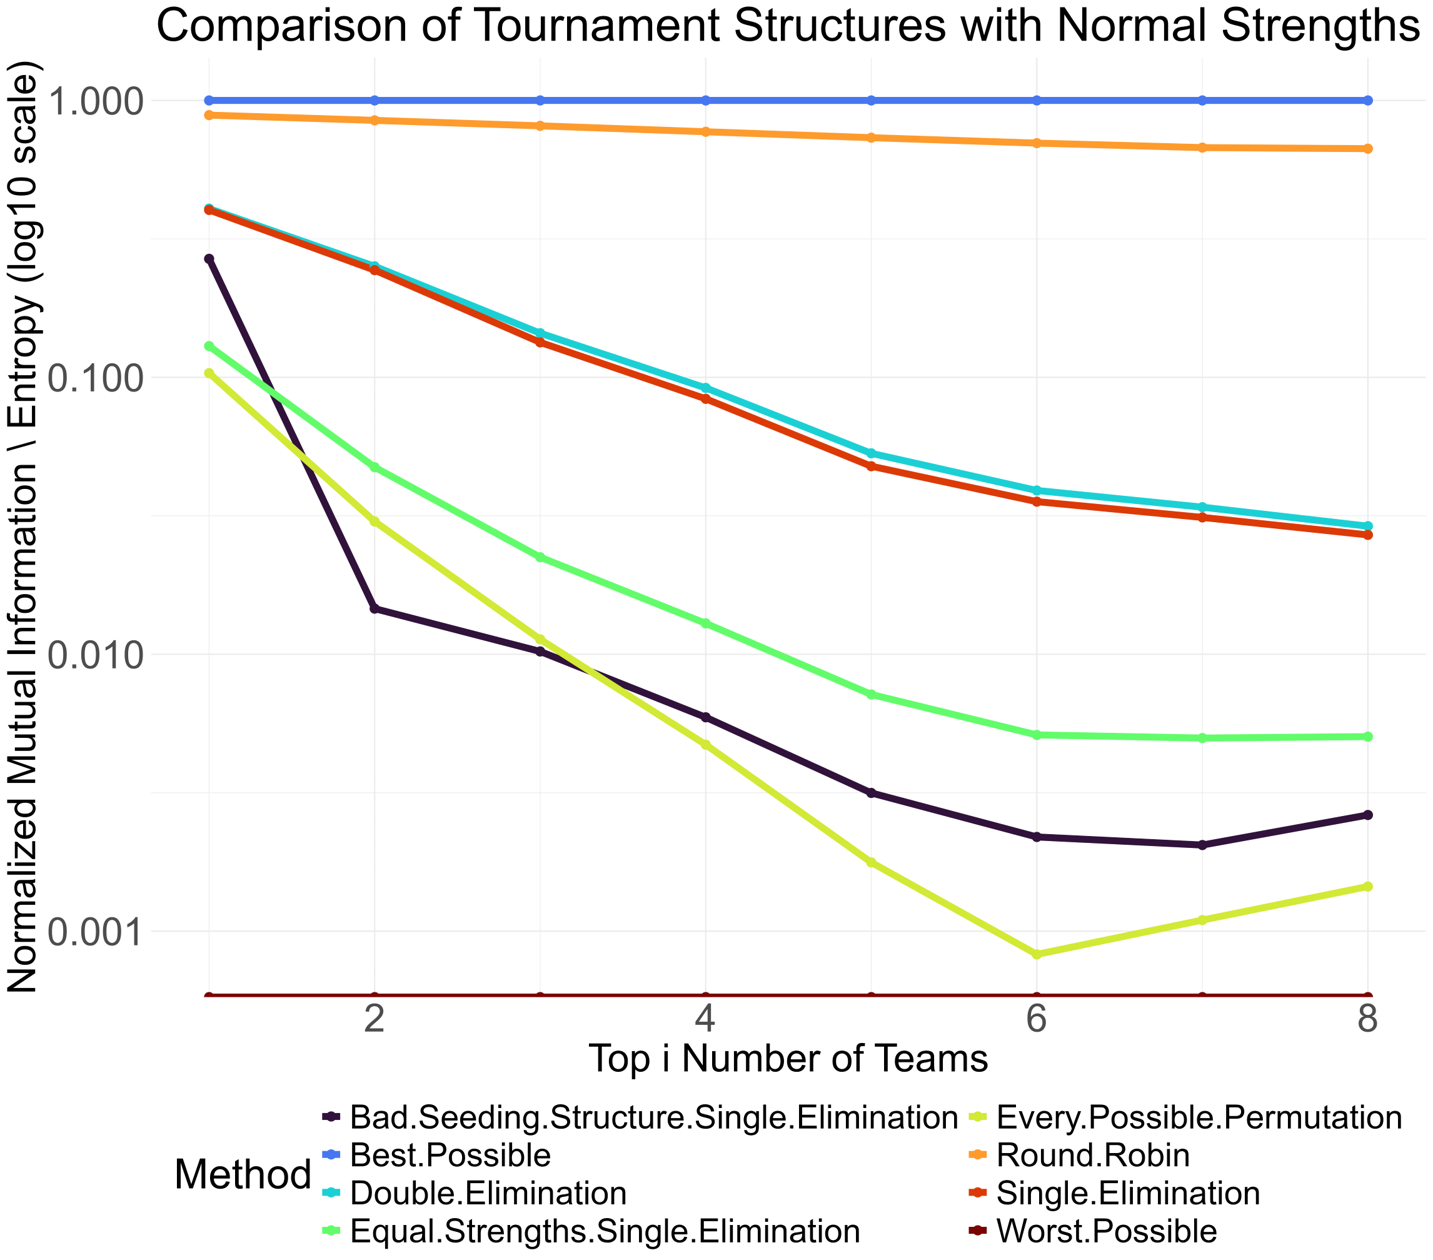
\includegraphics[width=4.25in,height=\textheight,keepaspectratio]{images/Normal_Information_Curve_Graph.png}
\caption{This figure compares the normalized weight mutual information
(on log10 scale) of various competition structures against the number of
salient ranks. \label{fig:fig1}}
\end{figure}

Figure \ref{fig:fig1} shows the results of the estimated values of
\(wI_m(r,\hat{r})\) on the y-axis (note the y-axis is on a \(log_{10}\)
scale) while the x-axis represents the number of salient weights that
were considered. Intuitively, of the competition structures considered
here, the round robin (shown in orange) should be the best as it
consists of the most match-ups by far of any structure considered here.
Note that it dominates all of the bracket structures regardless of the
choice of the number of salient ranks.

The single and double elimination bracket structures with traditional
seeding (red and light blue, respectively) are nearly identical and both
drastically better than the single elimination tournament with a bad
seeding structure (shown in black). The green curve preserves the
structure of a single elimination bracket and has the correct seeding,
but picks the winner based on a coin flip rather than weighting
simulated outcomes based on the strength of the competitors, whereas the
yellow curves shows results where every possible permutation of rankings
are equally likely. The green curve dominates the yellow curve here
because there are certain final rank orderings that are not possible in
bracket determined by coin flips because of the structure. So the
information that is generated from the tournament is based solely on the
seeding structure of the tournament. Whereas the yellow curve is based
on ranks generated from a tournament with essentially no structure at
all that happens to generate reasonable rankings occasionally.

Probably most notable in this figure is the black curve briefly dipping
below the yellow and green curves. What is happening here is that the
single elimination tournament with bad seeding (in black) is better when
the there is only a single salient rank. However, when the number of
salient ranks is 2, this drops \emph{below} the two curves that are
generates based on coin flip outcomes and completely random outcomes.
This is because in this structure the 1 and 2 seed both play each other
in the first round meaning that one of them will be eliminated
immediately. Thus under this seeding mechanism, the competition
structure simply cannot generate a correct result when the number of
salient ranks is 2. This structure is still below both green and yellow
curves when the number of salient ranks is 3, then recovers and climbs
above those curves when the number of salient ranks is 4 and continues
for the values of salient ranks 5 through 8.

\begin{figure}
\centering
\includegraphics[width=4.26042in,height=\textheight,keepaspectratio]{images/tournament_comparison_plot_se_de.png}
\caption{This figure focuses on the difference between single
elimination and double elimination competition structures
\label{fig:fig2}}
\end{figure}

Figure \ref{fig:fig2} shows the same red and light blue curves
representing single and double elimination, respectively, in more detail
as show in figure \ref{fig:fig1}. Note that in terms of declaring a
champion (i.e.~when the number of salient ranks is 1), single and double
elimination brackets are nearly identical is their ability to accomplish
this. However, double elimination is slightly better than single
elimination, with the gap growing wider as the number of salient ranks
increases. One clear reason for this is that with double elimination the
ranking of teams is ``clearer''. That is, in a single elimination
tournament the two teams that lose in the semi-finals can equally make a
claim as the third best team and in our schema they are randomly
assigned to a rank fo 3 or 4. However, in a double elimination
tournament, teams are definitively ranked 3 and 4 leading to beter
outcomes when the number of salient ranks is in the range of 3 to 4 (or
more).

\section{Conclusion}\label{sec:conclusion}

This study introduced a weighted mutual information framework to
evaluate the effectiveness of different competition formats in
preserving the true underlying rankings of teams. We also introduce the
concept of salient ranks, thereby extending and generalizing the
concepts of efficacy and effectivity. By simulating outcomes of
competition strucutres with varying seeding methods and applying an
information-theoretic approach, we quantified how accurately each format
conveys ranking information. Our findings confirm the intuitive
advantage of round robin tournaments, which consistently outperformed
single and double elimination formats in ranking accuracy, but also
quantify the difference between these structures. Additionally, we
demonstrated the degree to which poor seeding structures can
significantly degrade performance of a competition structure, in some
cases making competition outcomes even worse than simply randomly
generating a set of ranks.

These results underscore the trade-off between tournament accuracy and
practical constraints such as time, cost, and entertainment value. While
round robin offers the highest fidelity to true rankings, it is often
impractical for large tournaments, highlighting the need for hybrid or
adaptive structures that balance accuracy with logistical feasibility.

Future work should extend this analysis to scenarios with more
tournament structures, varying numbers of competitors, incorporate
probabilistic strength models reflecting real-world uncertainty, and
explore alternative weighting schemes for different competitive
priorities (e.g., 4 salient ranks versus 8 salient ranking). Applying
these methods to actual tournament data could further validate their
usefulness for organizers aiming to design fair and informative
competitions.

\section*{Acknowledgements}\label{acknowledgements}
\addcontentsline{toc}{section}{Acknowledgements}

We thank the Department of Mathematics and Statistics at Loyola
University Chicago for their support and resources in conducting this
study. We thank Kailey Marie Lum for the suggestion of the term
``salient ranks''. No external funding was received for this research.

\section*{Supplementary Material}\label{supplementary-material}
\addcontentsline{toc}{section}{Supplementary Material}

All supplementary material available at
\url{https://github.com/gjm112/tournaments}.

\section{References}\label{references}

\phantomsection\label{refs}
\begin{CSLReferences}{1}{0}
\bibitem[\citeproctext]{ref-Appleton1995-zn}
Appleton, David R. 1995. {``May the Best Man Win?''} \emph{Statistician}
44 (4): 529.

\bibitem[\citeproctext]{ref-Csato2021}
Csato, L. 2021. \emph{Tournament Design: How Operations Research Can
Improve Sports Rules. 1st Ed.} Cham, Switzerland: Palgrave Macmillan.

\bibitem[\citeproctext]{ref-Goosens2024}
Devriesere, Csató, K., and D. Goossens. 2025. {``Tournament Design: A
Review from an Operational Research Perspective.''} \emph{European
Journal of Operational Research} 324 (1): 1--21.

\bibitem[\citeproctext]{ref-Glenn1960-mn}
Glenn, W A. 1960. {``A Comparison of the Effectiveness of
Tournaments.''} \emph{Biometrika} 47 (3-4): 253--62.

\bibitem[\citeproctext]{ref-Guiasu1977-nu}
Guiasu, Silviu. 1977. \emph{Information Theory with Applications}. New
York, NY: McGraw-Hill.

\bibitem[\citeproctext]{ref-Johnson2022-wz}
Johnson, Sidney, and Rodney Fort. 2022. {``Match Outcome Uncertainty and
Sports Fan Demand: An Agnostic Review and the Standard Economic Theory
of Ports Leagues.''} \emph{Int. J. Emp. Econ.} 01 (02).

\bibitem[\citeproctext]{ref-Lasek2018-de}
Lasek, Jan, and Marek Gagolewski. 2018. {``The Efficacy of League
Formats in Ranking Teams.''} \emph{Stat. Modelling} 18 (5-6): 411--35.

\bibitem[\citeproctext]{ref-Sziklai2022-kf}
Sziklai, Balázs R, Péter Biró, and László Csató. 2022. {``The Efficacy
of Tournament Designs.''} \emph{Comput. Oper. Res.} 144 (105821):
105821.

\end{CSLReferences}

\end{document}
